% 2008 年安徽卷理科第 18 题：四棱锥 O-ABCD，底面菱形边长 1，∠ABC=π/4，
%   OA⊥底面，OA=2，M 为 OA 中点，N 为 BC 中点。
% 来源 PDF：gaokaomath-src/普通高考/2008/2008安徽理.pdf
% SHA-256：3493c8cb26596a78dafa0c1169fbdbfa4e69d8e593193f7c47128763b095c564
% 原页：2008安徽理.pdf 第 1 页（A3 三栏）第 3 栏，书页码 421。
% 重绘依据：按原页斜投影重绘：A 为被遮挡的后顶点，B 在左前、C 在右前、D 在右后；
%   A—B、A—D、A—O 用虚线，M、N 分别为 OA、BC 的中点，连 M—N、M—D 虚线。
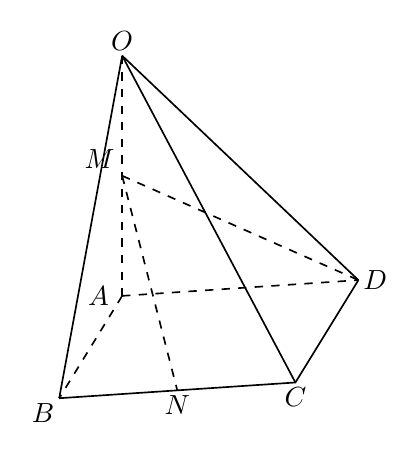
\begin{tikzpicture}[scale=1.0, semithick,
  every node/.style={inner sep=1.5pt}]

  \coordinate (B) at (0.40,0.75);
  \coordinate (C) at (3.40,0.95);
  \coordinate (D) at (4.20,2.25);
  \coordinate (A) at (1.20,2.05);
  \coordinate (O) at (1.20,5.10);
  \coordinate (M) at (1.20,3.575);
  \coordinate (N) at (1.90,0.85);

  % 底面：前棱与右棱可见，后两条棱被遮挡
  \draw (B) -- (C) -- (D);
  \draw[dashed] (A) -- (B);
  \draw[dashed] (A) -- (D);

  % 侧棱
  \draw (O) -- (B);
  \draw (O) -- (C);
  \draw (O) -- (D);
  \draw[dashed] (O) -- (A);

  % M 为 OA 中点，N 为 BC 中点
  \draw[dashed] (M) -- (N);
  \draw[dashed] (M) -- (D);

  \node[above] at (O) {$O$};
  \node[above left=1pt] at (M) {$M$};
  \node[left=3pt] at (A) {$A$};
  \node[below left] at (B) {$B$};
  \node[below] at (C) {$C$};
  \node[right] at (D) {$D$};
  \node[below] at (N) {$N$};
\end{tikzpicture}
